\chapter{Metodología}\label{metod}

\section{Metodología experimental}

\subsection{Plásmidos, reactivos, equipos y materiales}
La secuencia de los segmentos \ac{tm}-\ac{ic} de los péptidos $\alpha$IIb y $\beta$3 fueron donados por el laborario del Dr. Jun Qin {ref}. Cada plásmido fue clonado en la cepa de bacteria \ac{ecoli} DH5$\alpha$. La incorporación de los plásmidos fue verificada usando un kit de purificación de ADN "Wizard Plus SV Miniprep" (Promega, Madison, WI, USA). Ampicilina \hl{(escribir de donde se obtuvo, referencia)}   \ac{iptg} fue adquirido en Gentbiotech. Las  columnas  de Sefarosa Ni HisTrap HP  5 mL y de desalado PD-10 fueron adquiridas en GE Healthcare (Cat. 71-5027-68 Cat. 17085101, respectivamente). Para el \ac{hplc} se usó en equipo Agilent Technologies 1260 Infinity con detector de arreglo de diodos y longitud de onda múltiple (DAD VL), equipado con software ChemStation/Open LAB; columna Ultisil XB-C4, 5 $\mu$m, 300 Å, 4.6x250 mm, cat.00216-33043 (Welch SKU. H00216-33043, USA). Las membranas de celulosa (Dialysis Tubing, Benzoylated, poro de 2000 MWCO) fueron adquiridas en SIGMA. La concentración de proteína fue determina en espectrofotómetro Varian 2300, (Palo Alto, CA, USA). Las \ac{sds} y disoluciones amortiguadoras fueron preparadas usando agua grado Milli-Q tipo 1. Los análisis de \ac{em} se realizaron en un espectrómetro de masas ESI-Qq-TOF (Bruker). 
Los lípidos \ac{popc}, \ac{popg}, \ac{dppc}, fueron adquiridos en Avanti Polar, USA; el  \ac{chcl3}, \ac{acn} y \ac{meoh} grado \ac{hplc} en la firma Merck, Alemania.

\subsection{Extracción y clonación de plásmidos}
%%Para redactar ver parte se soporte del paper Qin & Jun
%%%https://www.sciencedirect.com/science/article/pii/S0168165622003042?via%3Dihub
%%% diagrama del plasmido https://sci-hub.se/10.1080/10409230490514008
Ambos plásmidos pMAL-c2 (New England Biolabs, Inc., Beverly, MA) fueron replicados por separado en la cepa \emph{E. coli} DH5$\alpha$ (ver \textbf{protocolo} \ref{Protocolo Plasmido}). Este vector contenía la secuencia que codifica cada péptido y la \ac{mbp} para facilitar un primer paso de purificación que llamaremos "proteína fusión". Entre el N-terminal de la \ac{mbp} y el C-terminal de cada péptido, hay una etiqueta de hexahistidina o His$_{6}$-\emph{tag} y sitio de corte para la proteasa del \ac{tev} que permiten separar cada secuencia de interés en dos pasos de purificación (\textbf{figura} \ref{fig:plasmido}). Además, posee la secuencia \emph{amp$^r$} que permite seleccionar bacterias que incorporen el plásmido con ampicilina. Todos los medios y material utilizado, asi como el agua Milli-Q fueron esterilizados en autoclave por 30 minutos a 1 atm de presión y 120°C.

%%%%%%%%%%%%%%%%%%%%% Fig plasmido %%%%%%%%%%%%%%%%%%%%%%%%
\begin{figure}[h] % supposedly places it here ...
    \centering
	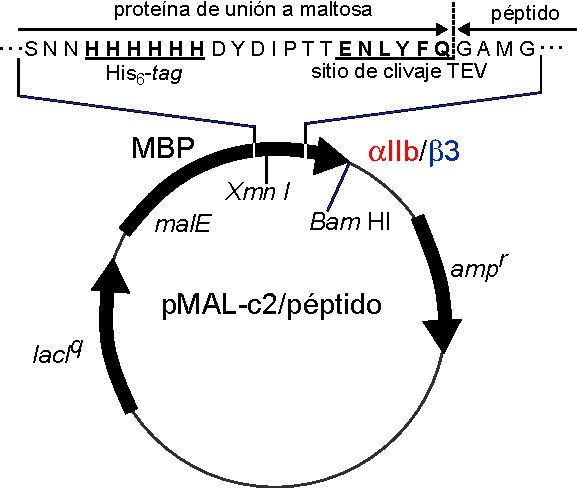
\includegraphics[width=0.79\linewidth]{fig/01_expe/pmal_c2.pdf}
	\caption[Esquema plásmido pMAL-c2 - $\alpha$IIb/$\beta$3]{Esquema plásmido pMAL-c2 - $\alpha$IIb/$\beta$3. Figura adaptada de Vector Database por \href{https://www.addgene.org/}{addgene.org} (2023). Extraído de \href{https://www.addgene.org/vector-database/3506/}{https://www.addgene.org/vector-database/3506/}.
        \index{plasmido}}
    \label{fig:plasmido}
\end{figure}
%%%%%%%%%%%%%%%%%%%%% Fin %%%%%%%%%%%%%%%%%%%%%%%%


\subsection{Expresión y purificación proteína fusión}\label{sec:expre_akta}

Una vez clonada cada secuencia \ac{tm}-\ac{ic} de los plásmidos $\alpha$IIb y $\beta$3 se expresó la proteína fusión en una cepa de bacterias \emph{E. coli} BL21(DE3), ver Protocolo \ref{Protocolo_Fusion}. Posteriormente se lisaron las bacterias y se purificó la proteína por afinidad a níquel en \ac{fplc}. 
Se cuantificó cada proteína fusión por espectrofotometría \ac{uv} teniendo en cuenta los coeficientes de absortividad molar, {\Large{$\varepsilon$}} a 280 nm: {\Large{$\varepsilon$}}$_{\alpha \text{IIb}}$ = 85830 M$^{\text{--1}}$ \, cm$^{\text{--1}}$, {\Large{$\varepsilon$}}$_{\beta\text{3}}$ = 83310 M$^{\text{--1}}$ \, cm$^{\text{--1}}$;
 valores obtenidos de \url{https://web.expasy.org/protparam/}. El rendimiento de cada \textbf{proteína fusión} fue de 10 y 15 mg/L cultivo para $\alpha$IIb y $\beta$3,  respectivamente.

Por otra parte también se expresó y purificó la proteasa \ac{tev} en nuestro laboratorio,  para ello, se tomó el plásmido de la proteasa TEV (donada por el laboratorio del Dr. Ernesto Ambroggio), se inoculó en la cepa \emph{E. coli} BL21(DE3) y se purificó por afinidad a níquel.

\subsection{Clivaje y diálisis}

La proteína fusión fue incubada con la proteasa \ac{tev} y se dejó a 30°C por $\Xapprox$ 48 horas. Se centrifugó y  se recuperó el sobrenadante el cual se dialisó en membranas de celulosa contra agua con agitación constante a 4°C. El contenido de las membranas se centrifugó en tubos eppendorf a 13000 \ac{rpm} por 10 minutos, \textbf{precipitando el péptido transmembrana} (en el sobrenadante se separó \ac{mbp}, \ac{tev} y proteína fusión sin cortar). El pellet se resuspendió \ac{acn}:H$_{2}$O 40:60 (vol/vol) con \ac{tfa}, consultar Protocolo \ref{Protocolo_TEV} para más detalle.

\subsection{Repurificación por \ac{hplc}}
Se realizaron múltiples cromatografías inyectando 1.0 mL de muestra bajo las siguientes condiciones cromatográficas:


%%%%%%%%%%%%%%%%%%%%% Tabla pequeña %%%%%%%%%%%%%%%%%%%%%%%%
\begin{wraptable}{r}{3.5cm}
\vspace{-0.8cm} %%%Posiciona a una altura en la hoja
\centering
    \caption{\\Gradiente HPLC.}\label{tab:hplc_gradiente}
    \begin{tabular}[t]{ccc}%%%c: center, l: leaft, r:right
     \toprule  % <-- Toprule here
      {Min}  & {A\%} & {B\%}\\
      \hline
        0       &  60    & 40  \\
        7       &  58    & 42 \\
        8       &  54    & 46  \\
        10      &  48    & 52 \\
        15      &  44    & 56  \\
        20      &  40    & 60 \\
        25      &  36    & 64  \\
        30      &  32    & 68 \\
        35      &  28    & 72  \\
    \textbf{40} & \textbf{24}    & \textbf{76} \\
        45      &  15    & 85  \\
        50      &  5     & 95 \\
        55      &  0     & 100  \\
      \bottomrule % <-- Bottomrule here
    \end{tabular}
    \vspace{-0.5cm} %%%Posiciona texto debajo tabla
    \end{wraptable} 
%%%%%%%%%%%%%%%%%%%%% Fin %%%%%%%%%%%%%%%%%%%%%%%%

\begin{tabularx}{\textwidth}{@{}p{0.20\textwidth} p{0.85\textwidth}@{}}
Fase móvil A: & 40\% H$_{2}$O(+0.1\% \ac{tfa}) \\
Flujo:              & 1.0 mL/min        \\ 
Temperatura:        & 40ºC              \\
Presión máxima:     & 210 bar           \\
Detector UV:        & 280 nm            \\
Inyección:          & 1.0 mL (manual)     \\
Fase móvil B:   & 100\% \ac{acn}(+0.1\% \ac{tfa}) \\
\end{tabularx}


Se colectaron todas fracciones del cromatograma según el gradiente de la \textbf{tabla} \ref{tab:hplc_gradiente} y se verificó la pureza por geles \ac{sds} y por \ac{em}.  Los péptidos purificados fueron solubilizados en \ac{acn}:H$_2$O 67\%/33\% (vol/vol); la concentración se determinó por absorbancia \ac{uv} teniendo en cuenta los {\Large{$\varepsilon$}} a 280 nm para cada péptido: {\Large{$\varepsilon$}}$_{\alpha \text{IIb}}$ = 16500 M$^{\text{--1}}$ cm$^{\text{--1}}$, {\Large{$\varepsilon$}}$_{\beta \text{3}}$ = 13980 M$^{\text{--1}}$ cm $^{\text{--1}}$. La remoción de \ac{tfa} y verificación de estructura secundaria de los péptidos se realizó por espectroscopía \ac{ftir}-\ac{atr}. El rendimiento final fue de 400 $\mu$g/L cultivo para $\alpha$IIb y 600 $\mu$g/L para $\beta$3. Se fraccionaron y almacenaron a -20°C para su posterior uso (ver Protocolo \ref{Protocolo_HPLC}).

\subsection{Electroforesis en gel y \ac{em}}

%%https://core.ac.uk/download/pdf/71054185.pdf
La pureza de ambos péptidos fue confirmada por geles SDS-PAGE y \ac{em}. Al tratarse de péptidos altamente hidrofóbicos se prepararon geles de poliacrilamida al 18\% en condiciones desnaturalizantes con \ac{sds}, junto con las muestras se sembró un marcador de peso molecular como referencia. La electroforesis se corrieron a 125 V y 4°C.

Se prepará una solución 100 $\mu$M de péptido en 67\%/33\% (vol/vol) + 0.1\% ácido fórmico y se inyectó en el espectrómetro de masas. El espectro fue adquirido en modo ion positivo desde 250 a 30000 m/z, con flujo de inyección de $\mu$L/min. El procesamiento de los datos se realizó en el software Data Analysis de Bruker \hl{REF}. Se promediaron dos cromatogramas, se procesó por deconvolución de la carga después de haber sustraído la línea base y se realizó un suavizado para obtener un cromatograma de alta resolución relación masa-carga m/z. Alternativamente los datos fueron post-procesados usando el Algoritmo de Máxima Entropía para obtener un espectro de masa neutra. Para ambos péptidos se obtuvo la masa esperada para los monómeros.

\subsection{Experimentos de monocapas de Langmuir}

Los experimentos de monocapas de Langmuir fueron realizados a temperatura ambiente (20°C). Todos los stock de soluciones de lípidos fueron preparadas en acetonitrilo:metanol. Las monocapas se realizaron en una unidad de control de Monofilmmeter (con Film Lift, Mayer Feintechnique, Alemania). La presión superficial ($\pi$) se midió usando el método de Wilhelmy con una placa Platinized-Pt y el potencial superficial ($\Delta$V) se detectó mediante el uso de una placa ionizante de $^{241}$Am. Los datos fueron registrados de forma continua y simultánea con un registrador X-YY de doble canal. El área superficial total de la cuba de Teflón fue de 80 cm$^2$ con capacidad de $\Xapprox$ 75 mL para la subfase (PBS 20 mM, NaCl 100 mM a pH 7.4). Para los péptidos puros se evaporó el solvente ACN:H$_2$O con flujo de nitrógeno (N$_{2 \text{(g)}}$) y se realizaron al menos 3 lavados con CHCl$_3$:MeOH 2:1 (vol/vol). La monocapa formaron directamente sembrando 0.5 nmoles de péptido solución CHCl$_3$:MeOH  en la subfase usando una jeringa Hamilton. Tanto para la isoterma del lípido puro como para las mezclas con péptidos se procedió de forma similar y se esperó por 8 minutos antes de empezar la compresión para dar tiempo a la evaporación del solvente y posteriormente se empezó a comprimir a razón fija de \hl{xx} cm$^2$/min. Antes de sembrar las muestras se realizaron los respectivos controles, para la superficie limpia y los disolventes de las muestras, en donde no se observó actividad superficial. Cada experimento se realizó por triplicado de forma independiente y se prepararon soluciones stock frescas de cada lípido cerca al momento de utilizarse.

Se realizaron ciclos de compresión-expansión, inicialmente las barreras se fijaron en 60 cm$^2$, se inició la compresión hasta llegar a los $\Xapprox$ 13 cm$^2$ y se expandió hasta los $\Xapprox$ 60 cm$^2$ y así se repitió tres veces para cada muestra.

%%%%Chequear este  \href{https://core.ac.uk/download/pdf/82003288.pdf}{link} para la discusión \href{https://reader.elsevier.com/reader/sd/pii/S0005273604000938?token=5AF045228C4131E3A6448735F6B35CEDFBE3138E3BF1D45DB2953593E8269614FD38EE1558AB7F2BBA9791113A5E77C5&originRegion=eu-west-1&originCreation=20230505170518}{otro link}

\subsection{Análisis de datos}

El procesamiento de los datos experimentales se realizó con código Python haciendo uso de las librerias  numpy (\hl{ref}), pandas (\hl{ref}). Todos los gráficos fueron generados con las librería Matplotlib (\hl{ref}).

%%Las imágenes de BAM fueron procesadas con el software Fiji (ref).

\section{Metodología computacional}

\subsection{Preparación de los sistemas}

%%https://ri.conicet.gov.ar/bitstream/handle/11336/80885/CONICET_Digital_Nro.9055fee5-f857-4ecf-960e-a5a4295f5f16_A.pdf;jsessionid=2EEA4DCEADDE4525930B5972D0F151B6?sequence=2

%%%https://ricabib.cab.cnea.gov.ar/952/1/1Cometto.pdf

%%https://bibliotecadigital.exactas.uba.ar/download/tesis/tesis_n6871_Bringas.pdf 
Las simulaciones de dinámica molecular grano grueso (CG-MD) se realizaron usando el campo de fuerza Martini 2 \hl{REF}, las coordenadas péptidos transmembrana fueron tomadas de la base de datos Protein Data Bank (PDB: 2KNC \hl{REF}. Se usó el servidor CHARMM-GUI \hl{REF} para emdidir el dímero $\alpha$IIb/$\beta$3 en una bicapa, el cual implementa el programa INSANE (INSert membrANE) que convierte las partículas del modelo atomístico a grano grueso \hl{REF}.
Los dinámicas se produjeron con los recursos de cómputo del \ac{sncad} usando los cluster Mendieta, Serafín (CCAD-UNC, \url{http://ccad.unc.edu.ar}) y con el cluster Create del King’s College London (\url{https://docs.er.kcl.ac.uk/CREATE/access/}). Se aplicó una red elástica aplicada (ElNeDyn) \hl{REF} sobre las partículas C$_\alpha$ de cada péptido usando una distancia \textit{cutoff} de 7 $\AA$, el dímero $\alpha$IIb/$\beta$3  fue insertado en 4 membranas de diferente composición cada una compuesta de 250 lípidos por hemicapa (POPC, POPG, POPC:POPG 70:30 (PCPG), DPPC). El sitema lípido-peptido fue hidratado con el modelo de agua polarizable (PW) \hl{REF}, finalmente se agregó NaCl hasta una concentración 0.15 M. El sistema se minimizó por 1000 pasos usando el método \textit{step desendent} \hl{REF}, posteriormente se equilibró en condiciones NPT por 5 ns aplicando posiciones de restricción para los $C_\alpha$ en las regiones con $\alpha$ hélice. Se usó el termostato de Berendsen \hl{REF} y el barostato Parrinello-Rahman \hl{REF} para mantener la temperatura a 320 K (excepto el sistema con DPPC que se simuló a 340 K) y la presión a 1 atmósfera con acoplamiento semi-isotrópico con una compresibilidad de 4.5 x 10$^{\text{--5}}$ bar$^{\text{--1}}$. Las interacciones eletrostáticas de largo alcance fueron incorporadas através del método de partículas de  Ewald con un \textit{cutoff} de 1 nm \hl{REF}. El mismo \textit{cutoff} se aplicó para las interacciones Lennard-Jones.


%%%REF insane: Wassenaar, T. A., Ingolfsson, H. I., Bockmann, R. A., Tieleman, D. P. & Marrink, S. J. Computational lipidomics with insane: A 
%%versatile tool for generating custom membranes for molecular simulations. J. Chem. Teory Comput. 11, 2144–2155 (2015).

%%%REF eledyn Lopez, C. A. et al. Martini coarse-grained force feld: Extension to carbohydrates. J. Chem. Teory Comput. 5, 3195–3210 (2009).
%%45. Periole, X., Cavalli, M., Marrink, S. J. & Ceruso, M. A. Combining an elastic network with a coarse-grained molecular force feld: 
%%Structure, dynamics, and intermolecular recognition. J. Chem. Teory Comput. 5, 2531–2543 (2009).


\subsection{Análisis de trayectorias}

El análisis de trayectorias se realizó con el paquete GROMACS, la librería MDAnalisys \hl{REF} con código en bash y python haciendo uso de algunas librerías como Numpy \hl{REF}, Pandas \hl{REF}. Los gráficos fueron generados con las librerías Matplotlib \hl{REF}, Seaborn \hl{REF}. La visualización de las trayectorias se realizó con el software VMD \hl{REF}.